\documentclass[
10pt, % Set the default font size, options include: 8pt, 9pt, 10pt, 11pt, 12pt, 14pt, 17pt, 20pt
%t, % Uncomment to vertically align all slide content to the top of the slide, rather than the default centered
aspectratio=169, % Uncomment to set the aspect ratio to a 16:9 ratio which matches the aspect ratio of 1080p and 4K screens and projectors
]{beamer}

\usepackage[all]{xy}

\usepackage[spanish]{babel}
\usepackage[utf8]{inputenc}

\graphicspath{{Images/}{./}} % Specifies where to look for included images (trailing slash required)

\usepackage{booktabs} % Allows the use of \toprule, \midrule and \bottomrule for better rules in tables

%\usepackage{tikz}
%\usetikzlibrary{positioning}
%\usetikzlibrary{shapes,arrows,arrows,positioning,fit}

\usepackage{tikz}
\usepackage{adjustbox}
\usetikzlibrary{arrows, shapes}

\usepackage{forest}

\usepackage{multirow}

\usepackage{graphicx}
\usepackage{hyperref}

\usepackage{xcolor,listings}
\usepackage{textcomp}
%\usepackage{color}

\usepackage{enumitem}

\usepackage{xcolor}

\usepackage{verbatim}
\usepackage{changepage}

\usepackage{algpseudocode}
\usepackage{gensymb}

\usepackage{venndiagram}

\usepackage{graphicx}

\usepackage{array}

\usepackage{colortbl}


% \usepackage{media9}

% \usepackage{algorithm}
% \usepackage{algorithmic}

\providecommand{\abs}[1]{\lvert#1\rvert}

%----------------------------------------------------------------------------------------
%	SELECT LAYOUT THEME
%----------------------------------------------------------------------------------------
\usetheme{Madrid} 

%----------------------------------------------------------------------------------------
%	SELECT COLOR THEME
%----------------------------------------------------------------------------------------
%\usecolortheme{beaver}
%\usecolortheme{seahorse}
\usecolortheme{spruce} % verde suave
%\usecolortheme{whale}
%\usecolortheme{wolverine}

%----------------------------------------------------------------------------------------
%	SELECT FONT THEME & FONTS
%----------------------------------------------------------------------------------------
\usefonttheme{default} % Typeset using the default sans serif font
%\usefonttheme{serif} % Typeset using the default serif font (make sure a sans font isn't being set as the default font if you use this option!)
%\usefonttheme{structurebold} % Typeset important structure text (titles, headlines, footlines, sidebar, etc) in bold
%\usefonttheme{structureitalicserif} % Typeset important structure text (titles, headlines, footlines, sidebar, etc) in italic serif
%\usefonttheme{structuresmallcapsserif} % Typeset important structure text (titles, headlines, footlines, sidebar, etc) in small caps serif

%------------------------------------------------

%\usepackage{mathptmx} % Use the Times font for serif text
%\usepackage{palatino} % Use the Palatino font for serif text

\usepackage{helvet} % Use the Helvetica font for sans serif text
%\usepackage[default]{opensans} % Use the Open Sans font for sans serif text
%\usepackage[default]{FiraSans} % Use the Fira Sans font for sans serif text
\usepackage[default]{lato} % Use the Lato font for sans serif text

%----------------------------------------------------------------------------------------
%	SELECT INNER THEME
%----------------------------------------------------------------------------------------
\useinnertheme{circles}


\setbeamertemplate{footline} % Uncomment this line to remove the footer line in all slides
%\setbeamertemplate{footline}[page number] % Uncomment this line to replace the footer line in all slides with a simple slide count

\setbeamertemplate{navigation symbols}{} % Uncomment this line to remove the navigation symbols from the bottom of all slides

%----------------------------------------------------------------------------------------
%	PRESENTATION INFORMATION
%----------------------------------------------------------------------------------------

\title[Short Title]{Minería en la web: búsqueda, crawling y scraping} 

\subtitle{Sistemas de Recuperación de Información}

\author{Lic. Carlos León González \\ Dra.C. Lucina García Hernández}

\institute[UC]{Facultad de Matem\'atica y Computaci\'on \\ Universidad de La Habana \\ \smallskip }

\date{4 de marzo de  2024} % Presentation date or conference/meeting name, the optional parameter can contain a shortened version to appear on the bottom of every slide, while the required parameter value is output to the title slide

%----------------------------------------------------------------------------------------

\begin{document}
	
	\lstset{
		literate=%
		{á}{{\'a}}1
		{í}{{\'i}}1
		{é}{{\'e}}1
		{ý}{{\'y}}1
		{ú}{{\'u}}1
		{ó}{{\'o}}1
		{ě}{{\v{e}}}1
		{š}{{\v{s}}}1
		{č}{{\v{c}}}1
		{ř}{{\v{r}}}1
		{ž}{{\v{z}}}1
		{ď}{{\v{d}}}1
		{ť}{{\v{t}}}1
		{ň}{{\v{n}}}1                
		{ů}{{\r{u}}}1
		{Á}{{\'A}}1
		{Í}{{\'I}}1
		{É}{{\'E}}1
		{Ý}{{\'Y}}1
		{Ú}{{\'U}}1
		{Ó}{{\'O}}1
		{Ě}{{\v{E}}}1
		{Š}{{\v{S}}}1
		{Č}{{\v{C}}}1
		{Ř}{{\v{R}}}1
		{Ž}{{\v{Z}}}1
		{Ď}{{\v{D}}}1
		{Ť}{{\v{T}}}1
		{Ň}{{\v{N}}}1                
		{Ů}{{\r{U}}}1    
	}
	
	
	\begin{frame}
		\titlepage
	\end{frame}
	
	%------------------------------------------------
	% Objetivos
	\begin{frame}
		
		\frametitle{Objetivos}
		
		\begin{itemize}

			\item Identificar y caracterizar las distintas etapas del desarrollo de la Web.
			
			\item Abordar los distintos componentes de un motor de Recuperación de Información en la Web.
			
			\item Definir las funciones del crawler y el scraper.
						
		\end{itemize}
		
	\end{frame}
	
	%------------------------------------------------
	% Duda
	\begin{frame}
		
		\frametitle{Duda}
		
		\centering 
		
		\textcolor{purple}{
			¿Representan lo mismo?
		} 
		
		\vspace{1\baselineskip}
		
		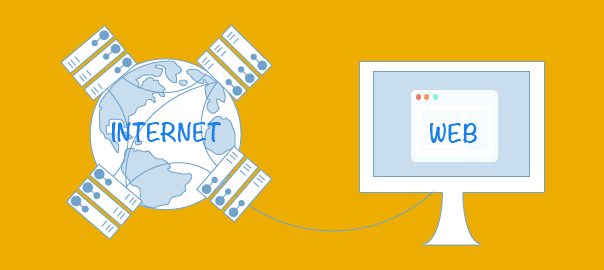
\includegraphics[scale=0.5]{internet-web.png} \\[2mm]
		
		{\scriptsize Tomado de \url{https://ladiferenciaentre.info/internet-web/}}
		
	\end{frame}
	
	%------------------------------------------------
	% Diferencias entre Internet y Web
	\begin{frame}[fragile]
		
		\frametitle{Diferencias entre Internet y Web}
		
		\begin{centering}
			
			\begin{tabular}{|p{5.2cm}|p{2.6cm}|p{5.2cm}|}
				\hline
				
				\rowcolor{lightgray}
				\textbf{Internet} & \textbf{Comparativa} & \textbf{Web} \\ \hline
				\hline
				
				Infraestructura de comunicación 
				& \cellcolor{lightgray} ¿Qué es? 
				& Conjunto de documentos conectados a través de hipertexto. \\ 
				\hline
				
				ARPANET fue la primera red de computadoras. Creada por el Departamento de Defensa de EE.UU. en 1968.
				& \cellcolor{lightgray} Creación
				& La primera propuesta de la web fue presentada por Tim Berners-Lee en el CERN en 1989. \\ 
				% El CERN es la Organización Europea para la Investigación Nuclear y es uno de los centros de investigación más importantes del mundo.
				\hline
				
				Funciona con el protocolo TCP/IP que divide los datos en paquetes y los une en el destino 
				& \cellcolor{lightgray} ¿Cómo funciona? 
				& Los documentos se codifican en HTML y se envía a través del protocolo HTTP \\ 
				\hline
								
			\end{tabular}
	
		\end{centering}
		
	\end{frame}
	
	%------------------------------------------------
	% Diferencias entre Internet y Web
	\begin{frame}[fragile]
		
		\frametitle{Diferencias entre Internet y Web}
		
		\begin{centering}
			
			\begin{tabular}{|p{5.2cm}|p{2.6cm}|p{5.2cm}|}
				\hline
				\rowcolor{lightgray}
				\textbf{Internet} & \textbf{Comparativa} & \textbf{Web} \\ \hline
				\hline
				
				\begin{itemize}
					\item Descentralizada 
					\item Abierta 
					\item Escalable 
					\item Diversidad de protocolos
				\end{itemize}
				& \cellcolor{lightgray} Ventajas 
				& \begin{itemize}
					\item Acceso mediante hipervínculos 
					\item Navegación por páginas web 
					\item Interactividad
					% La interactividad se refiere a la capacidad de un sistema o dispositivo de responder a las acciones del usuario y permitir una comunicación bidireccional.
				\end{itemize} \\ 
				\hline
			
				\begin{itemize}
					\item Acceso no garantizado 
					\item Vulnerabilidad a ataques 
					\item Congestión 
					\item Falta de control
				\end{itemize}
				& \cellcolor{lightgray} Desventajas
				& 	\begin{itemize}
					\item Dependencia de Internet 
					\item Requiere software específico 
					\item Contenido no siempre veraz 
					\item Limitaciones de accesibilidad
				\end{itemize} \\
				\hline
				
			\end{tabular}
			
		\end{centering}
		
	\end{frame}
	
	%------------------------------------------------
	% Pero ...
	\begin{frame}
		
		\frametitle{Pero ...}
		
		\only<1>{
			\begin{centering}
				
				\textcolor{purple}{
					¿Siempre la Web ha sido igual? \\
					¿Ha sufrido algún cambio?
				}
			
			\end{centering}
		}
		
		\only<2>{
			La Web ha sufrido cambios desde su surgimiento a finales de la década de 1980 y se ha dividido en distintas eras.
		}		
		
	\end{frame}
	
	%------------------------------------------------
	% Web 1
	\begin{frame}
		
		\frametitle{Era: Web 1.0}
		
		Características:
		\begin{itemize}

			\item Comunicación unidireccional
			%Los propietarios de los sitios web proporcionaban contenido y los usuarios lo consumían de forma pasiva.
			
			\item Interacción limitada del usuario
			%Los usuarios tenían una capacidad limitada para interactuar con sitios web más allá de la navegación básica y hacer clic en enlaces.
		
			\item Sitios web estáticos
			%Los sitios eran predominantemente estáticos. Las actualizaciones requerían la edición manual del código HTML (del inglés HyperText Markup Language).
			
			\item Falta de interacción social
			%Las redes sociales y el contenido generado por los usuarios eran prácticamente inexistentes. Los sitios web se centraron en brindar información en lugar de facilitar la colaboración o participación de los usuarios.
		
			\item Ausencia de contenido dinámico  
			%Carecía de contenido dinámico, experiencias personalizadas y actualizaciones en tiempo real.
			
		\end{itemize}
		
		\centering
		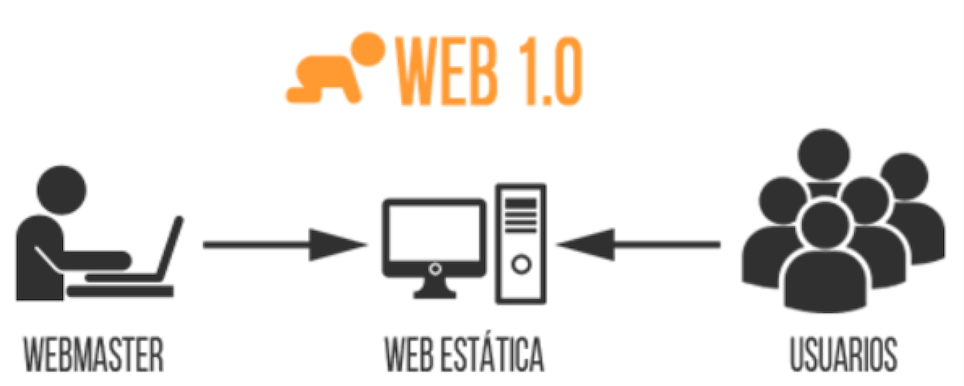
\includegraphics[scale=0.53]{web1_0.png} \\[2mm]
		
		{\scriptsize Tomado de \url{https://laeradigitaltierno.home.blog/2019/01/17/3-1-evolucion-de-la-web/}}
		
		% 
		% Ejemplos: 
		% 
		% 	- CNN: en sus primeras versiones representa esta era. Sitio de noticias. 
		% 	
		% 	- Amazon (1995): Amazon comenzó como una librería en línea en 1995. Ofrecía una interfaz simple para buscar y comprar libros.
		% 	
		% 	- Yahoo! (1994): Uno de los primeros motores de búsqueda y directorios web. Su sitio web en sus primeras versiones ofrecía una lista organizada de enlaces a recursos de Internet.
		% 
		
	\end{frame}
	
	%------------------------------------------------
	% Web 1.5
	\begin{frame}
		
		\frametitle{Web 1.5}
		
		Puede considerarse que la incorporación de las bases de datos en los sitios web estáticos de la \textbf{Web 1.0} es un paso superior, dándose la \textbf{Web 1.5}.\\[2mm]
		
		El uso de las bases de datos por los sitios web tenía como objetivo atraer más usuarios en la red. 
		
		\pause
		\vspace{3\baselineskip}
		
		La \textbf{Web 1} se conoce también como \textbf{Web de solo lectura} o \textbf{Web estática}.
		
	\end{frame}
	
	%------------------------------------------------
	% Web 2.0
	\begin{frame}
		
		\frametitle{Era: Web 2.0}
		
		En 2004 Tim O'reilly introduce el concepto de Web 2.0, difiniéndolo como:
		
		\begin{alertblock}{}
			Un conjunto de aplicaciones donde el usuario tiene el control y se caracterizan por estar basadas en la inteligencia colectiva y el uso de servicios interactivos en red.
		\end{alertblock}
		

		
	\end{frame}
	
	%------------------------------------------------
	% Web 2.0
	\begin{frame}
		
		\frametitle{Era: Web 2.0}
		
		Características:
		\begin{itemize}
			
			\item Contenido generado por el usuario
			%Las plataformas permite a los usuarios crear, compartir y modificar contenido, resultando un aumento significativo en la participación y colaboración de los usuarios.
			
			\item Interactividad y participación
			% Existencia de sitios web dinámicos e interactivos que permitieron a los usuarios participar, comentar e interactuar tanto con los creadores de contenido como con otros usuarios.
			
			\item Uso de plataformas sociales
			%El auge de las plataformas de redes sociales como Facebook, Twitter y YouTube definió esta era, permitiendo a los usuarios conectarse, compartir y comunicarse entre sí a escala global.
			
			\item Aplicaciones enriquecidas de Internet (AJAX, JavaScript, Flash)
			%Aprovechando tecnologías como AJAX, JavaScript y Flash para crear experiencias web más interactivas y con mayor capacidad de respuesta.
			
			\item Personalización y adaptación
			%Las plataformas ofrecían experiencias personalizadas, lo que permitía a los usuarios personalizar sus perfiles, recibir recomendaciones de contenido personalizadas y participar en filtrado colaborativo.
			
		\end{itemize}
		
		\centering
		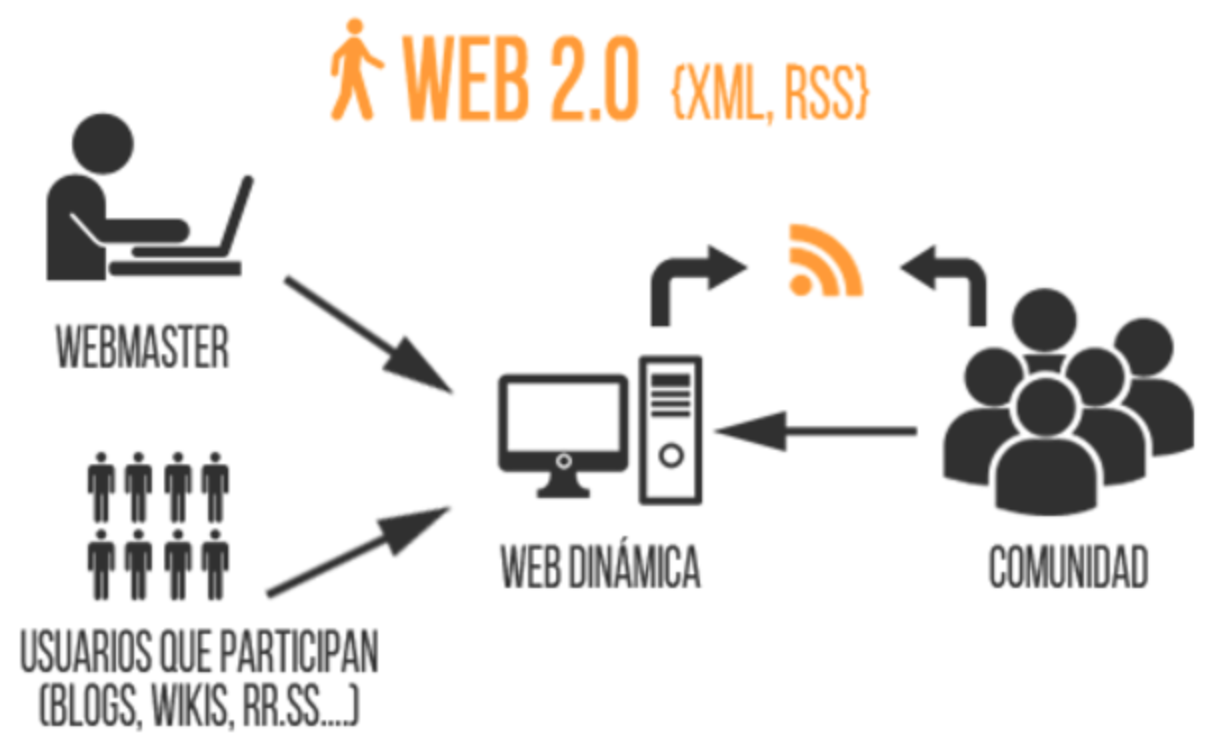
\includegraphics[scale=0.37]{web2_0.png} 
		
		{\scriptsize Tomado de \url{https://laeradigitaltierno.home.blog/2019/01/17/3-1-evolucion-de-la-web/}}
		
		% XML, que significa "Extensible Markup Language" (Lenguaje de Marcado Extensible), es un lenguaje de marcado que define un conjunto de reglas para codificar documentos de manera legible tanto para humanos como para máquinas. Fue diseñado para ser extensible y adaptable a una amplia variedad de aplicaciones.
		
		% RSS significa "Really Simple Syndication" (Sindicación Realmente Simple). Es un formato de fuente web que permite a los usuarios acceder y distribuir contenido actualizado de manera sistemática desde sitios web que cambian con frecuencia, como blogs, noticias, podcasts y otros medios en línea.
		
	\end{frame}
	
	%------------------------------------------------
	% Aplicación Web
	\begin{frame}
		
		\frametitle{Avances en las aplicaciones web}
		
		\begin{minipage}[t]{0.4\textwidth} % Primera columna
			
			\centering 
			\textbf{Web 1}\\[2mm]
			
			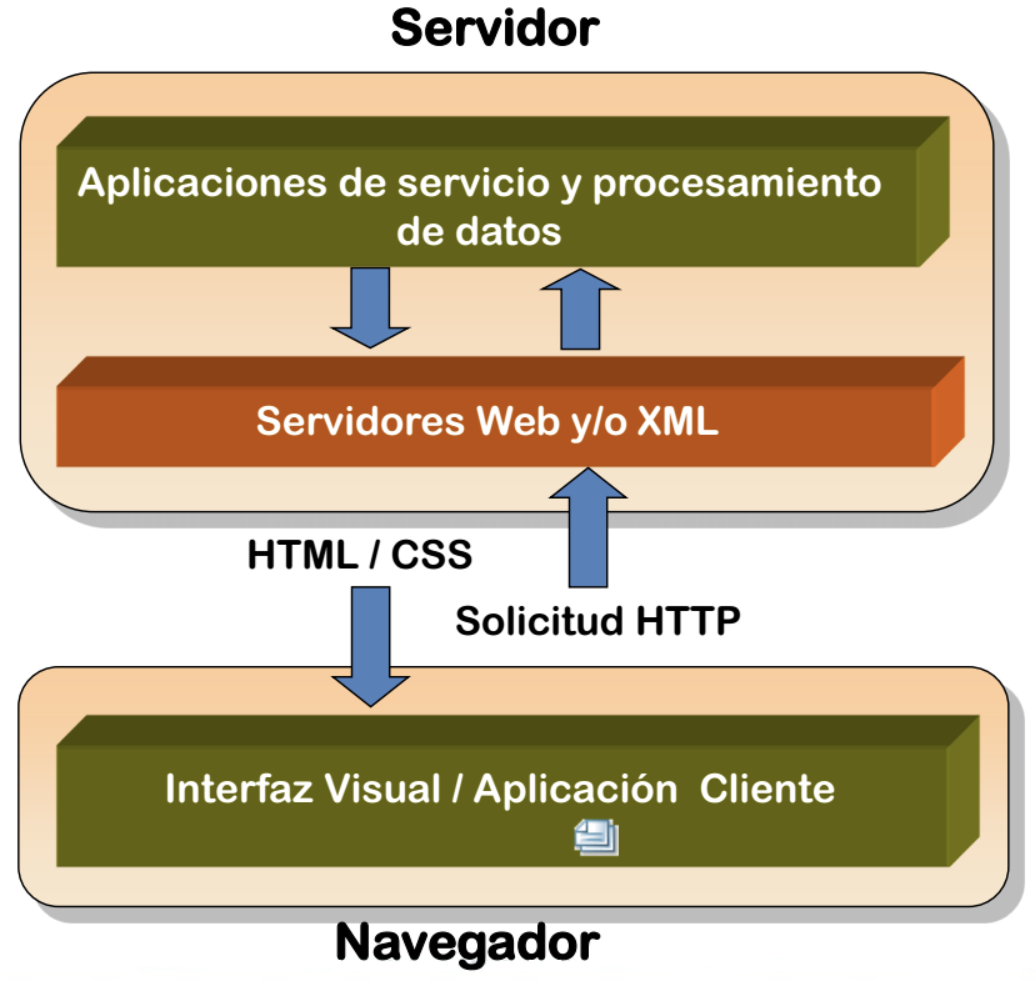
\includegraphics[scale=0.35]{modelo-web1.png} 
			
		\end{minipage}
		\hfill  % Espacio entre las columnas
		\begin{minipage}[t]{0.4\textwidth} % Segunda columna
			
			\centering 
			\textbf{Web 2}\\[2mm]
			
			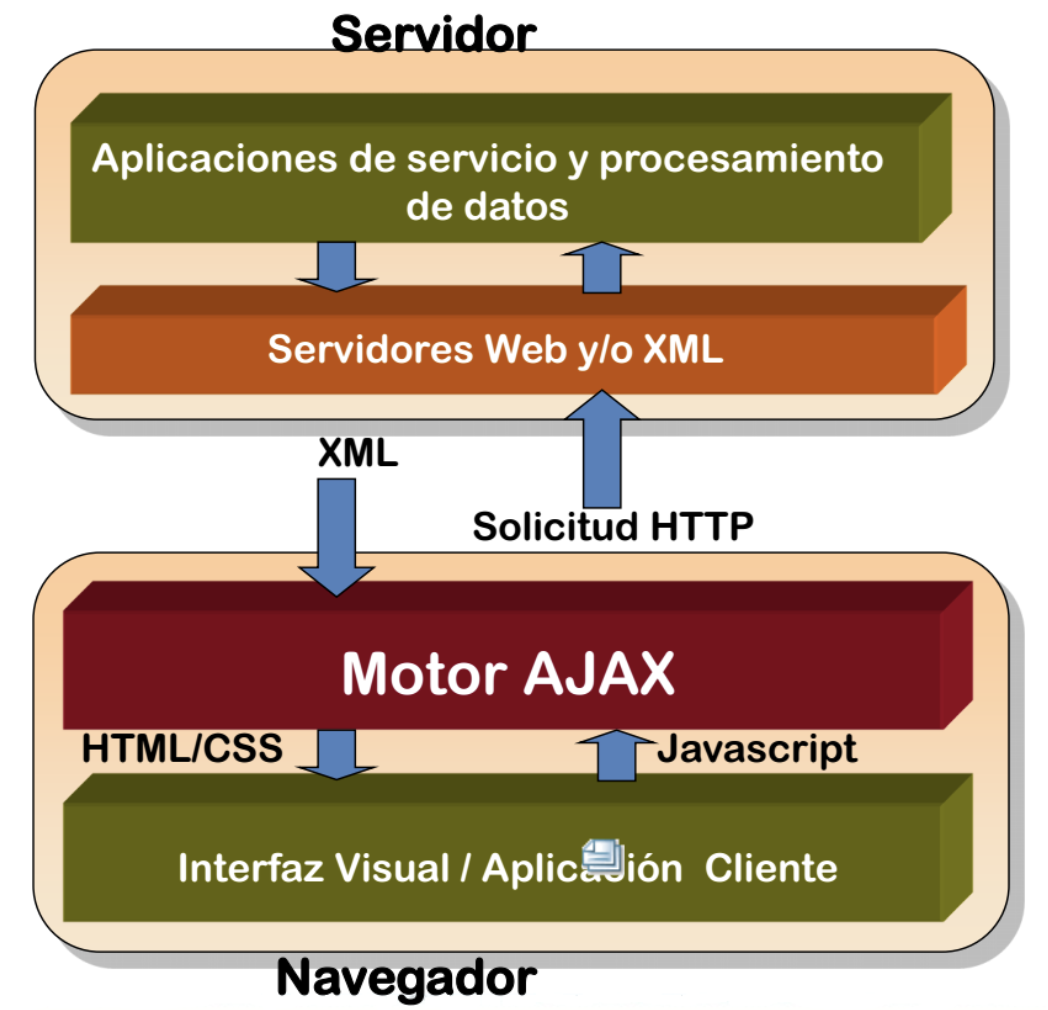
\includegraphics[scale=0.35]{modelo-web2.png} 
			
		\end{minipage}
		
	\end{frame}
	
	%------------------------------------------------
	% Necesidad
	{
		\setbeamertemplate{background canvas}
		{%
			
\includegraphics[width=\paperwidth,height=\paperheight]{necesidad.png}
		}
		
		\begin{frame}
		\end{frame}
	}
	
	%------------------------------------------------
	% Web 2.5
	\begin{frame}
		
		\frametitle{Web 2.5}
		
		 La incorporación de las redes sociales, la popularización de los usuarios y las entidades y la comunidad virtual generadas crean una transición a una era de la web con mayor especialización: \textbf{Web 2.5}. \\[2mm]
		
		\begin{centering}
			
			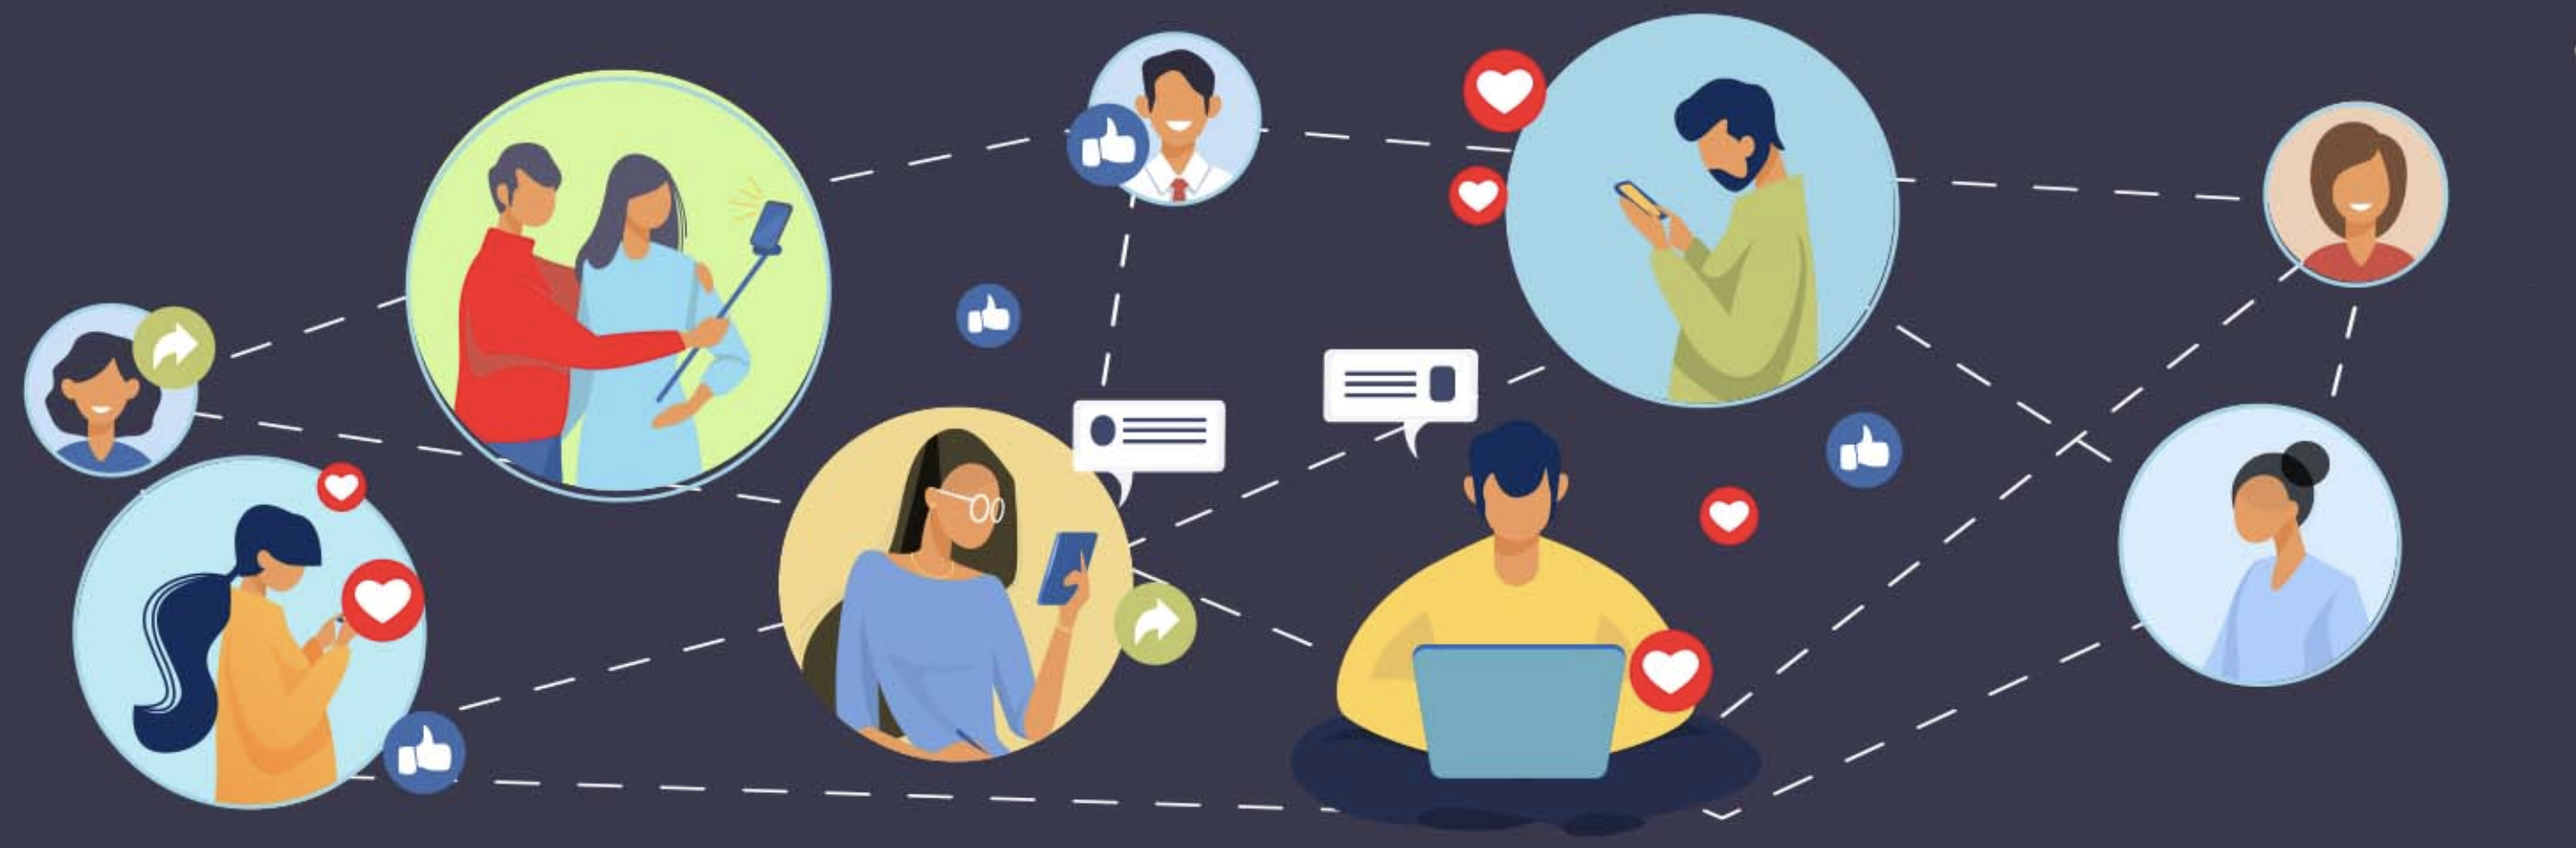
\includegraphics[scale=0.2]{comunidad.png} 
			
			{\scriptsize Tomado de \url{https://www.nunify.com/blogs/build-virtual-communities-around-virtual-events/}} 
			
		\end{centering}
		
		\vspace{0.8\baselineskip}
		
		\begin{alertblock}{Comunidad virtual}
			Conjunto de individuos que con un mismo objetivo o propósito se unen para coincidir en una Red Social Virtual apoyándose en tecnologías que permiten realizar esta relación de forma virtual.
		\end{alertblock}
		
		% Si no apareces en una red social, no eres importante
		
	\end{frame}
	
	%------------------------------------------------
	% Problemas de la Web 2
	\begin{frame}
		
		\frametitle{Web 2}
		
		La \textbf{Web 2} se conoce también como \textbf{Web de escritura-lectura} o \textbf{Web social}.
		
	\end{frame}
	
	%------------------------------------------------
	% Problemas de la Web 2
	\begin{frame}
		
		\frametitle{Problemas de la Web 2}
		
		\begin{itemize}
			\item Diseñada para el uso humano
			\item Crecimiento por segundo del volumen de información disponible
			\item Evoluciona como un repositorio caótico
			\item Diseño no adecuado para la publicación y recuperación de información de manera ``organizada''
			\item Resultados irrelevantes en las búsquedas
			\item Web totalmente sintáctica
		\end{itemize}
		
		\vspace{2\baselineskip}
		\pause
		\textcolor{purple}{
			¿Qué hacer para intentar dar significado dentro de la Web?
		}
		
	\end{frame}
	
	%------------------------------------------------
	% Web semántica
	\begin{frame}
		
		\frametitle{Web semántica}
		
		En 2001 se propuso por el propio creador de la web, Tim Berners-Lee, un nuevo rasgo para añadir en la web, siendo: 
		
		\begin{alertblock}{Web semántica}
			Es una extensión de la web actual (Web 2.0) en la cual la información recibe un significado bien definido, permitiendo a los computadores y las personas trabajar en cooperación de mejor forma.
		\end{alertblock}
		
		% Consiste en la adhesió de metadatos semánticos a los sitios web que describen el contenido, el significado y la relación entre los datos. 
		
		\vspace{2\baselineskip}
		Su objetivo es que la web sea más comprensible para los agentes de búsqueda en términos de relevancia y precisión.
		
	\end{frame}
	
	%------------------------------------------------
	% Web 3
	\begin{frame}
		
		\frametitle{Web 3}
		
		\begin{itemize}
			
			\item Descentralización y tecnología Blockchain 
			% Aprovecha las redes descentralizadas, la tecnología blockchain y los contratos inteligentes para permitir interacciones entre pares, transacciones seguras y aplicaciones descentralizadas.
			
			\item Control del usuario y propiedad de los datos 
			% Hace hincapié en brindar a los usuarios un mayor control sobre sus datos, identidades digitales e interacciones en línea. Su objetivo es desviar el poder de las entidades centralizadas hacia los usuarios individuales.
			
			\item Privacidad y seguridad mejoradas 
			%Se centra en mejorar la privacidad y la seguridad aprovechando el cifrado, el almacenamiento descentralizado y las tecnologías que preservan la privacidad.
			
			\item Interoperabilidad e integración perfecta 
			%Tiene como objetivo establecer la interoperabilidad entre diferentes redes y protocolos de blockchain, permitiendo una comunicación fluida, el intercambio de datos y la transferencia de valor entre plataformas.
			
			\item Integración inteligente de la Web y la IA 
			%Prevé la integración de tecnologías de inteligencia artificial (IA), aprendizaje automático y procesamiento del lenguaje natural para mejorar las capacidades de búsqueda, la curación de contenidos y las experiencias de los usuarios.
			
			\item Espacios tridimencionales 
			
		\end{itemize}
		
		\centering
		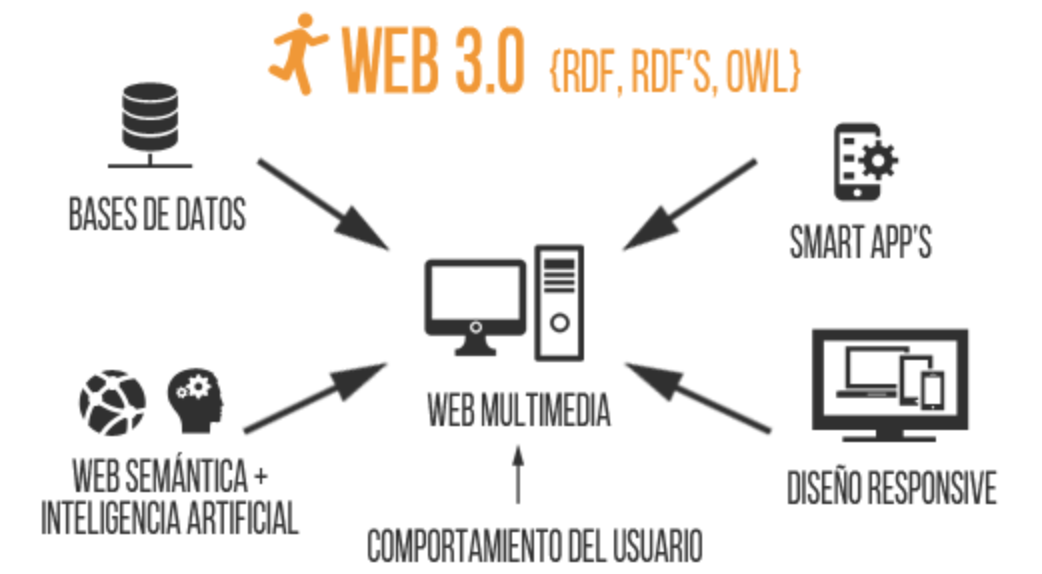
\includegraphics[scale=0.37]{web_3.png} 
		
		{\scriptsize Tomado de \url{https://laeradigitaltierno.home.blog/2019/01/17/3-1-evolucion-de-la-web/}}
		
		% RDF (Resource Description Framework): Ees un marco de trabajo estándar para describir recursos y sus relaciones en la web. Permite representar la información en forma de declaraciones triples: sujeto, predicado y objeto. Estos triples forman un grafo dirigido que representa la información de manera estructurada y semántica. RDF se utiliza para representar metadatos, ontologías, vocabularios y datos estructurados en la web semántica. Es una parte fundamental de la infraestructura que permite la interoperabilidad y el intercambio de datos entre diferentes sistemas y aplicaciones en la web.
		
		%OWL (Web Ontology Language): Es un lenguaje de ontología basado en RDF que permite definir ontologías y describir relaciones entre conceptos en la web semántica. Proporciona un conjunto más rico y expresivo de constructos para la descripción de ontologías que RDF, incluyendo clases, propiedades, restricciones y axiomas. OWL se utiliza para modelar y representar el conocimiento en dominios específicos, permitiendo la creación de ontologías formales que capturan la semántica de un dominio y facilitan el razonamiento automático sobre la información.
		
	\end{frame}
	
	%------------------------------------------------
	% Posterior a Web 3 ...
	\begin{frame}
		
		\frametitle{Posterior a Web 3 ...}
		
		%No ha sido planteada de forma formal, pero será como estar en un espacio inteligente en el que no será necesario preguntarle al buscador. Será una web interoperable en la que se le harán planteamientos a dispositivos inteligentes que se vincularán con los sistemas recuperadores de información para obtener respuestas a iterrogaciones concretas. 
		
		\centering
		
		Conocida como \textbf{Web simbólica}
		
		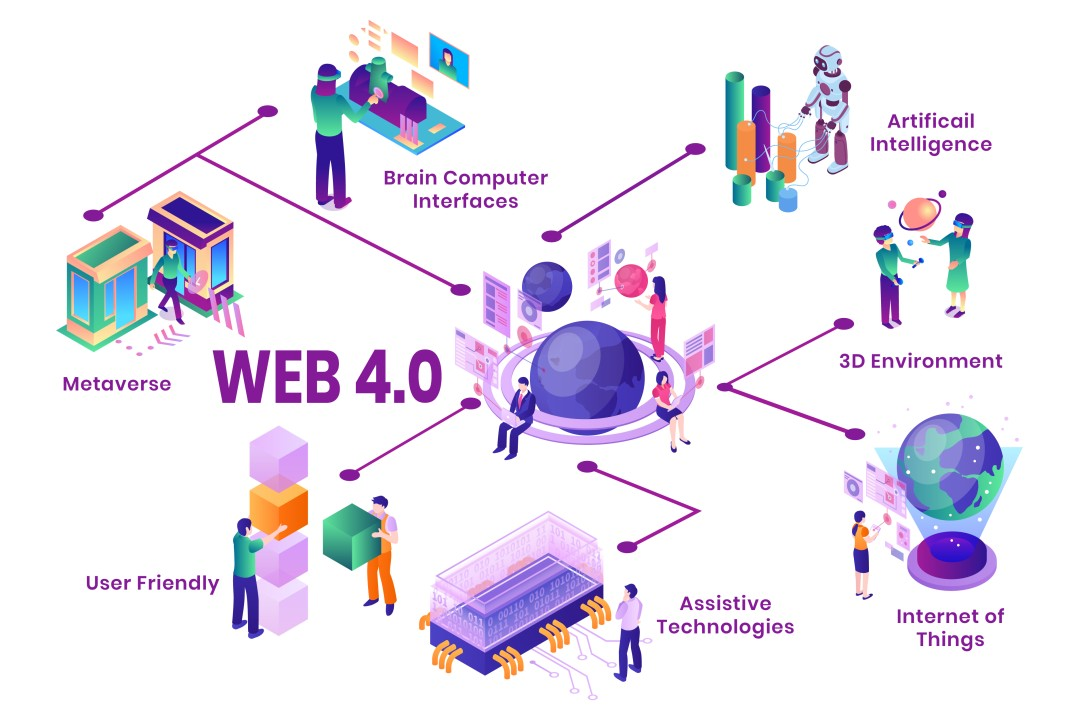
\includegraphics[scale=0.25]{web_4.jpeg} 
		
		{\scriptsize Tomado de \url{https://www.linkedin.com/pulse/web-40-explained-brief-agiledistrict/}}
		
	\end{frame}
	
	%------------------------------------------------
	% Evolución de la web
	\begin{frame}
		
		\frametitle{Evolución de la web}
		
		\centering
		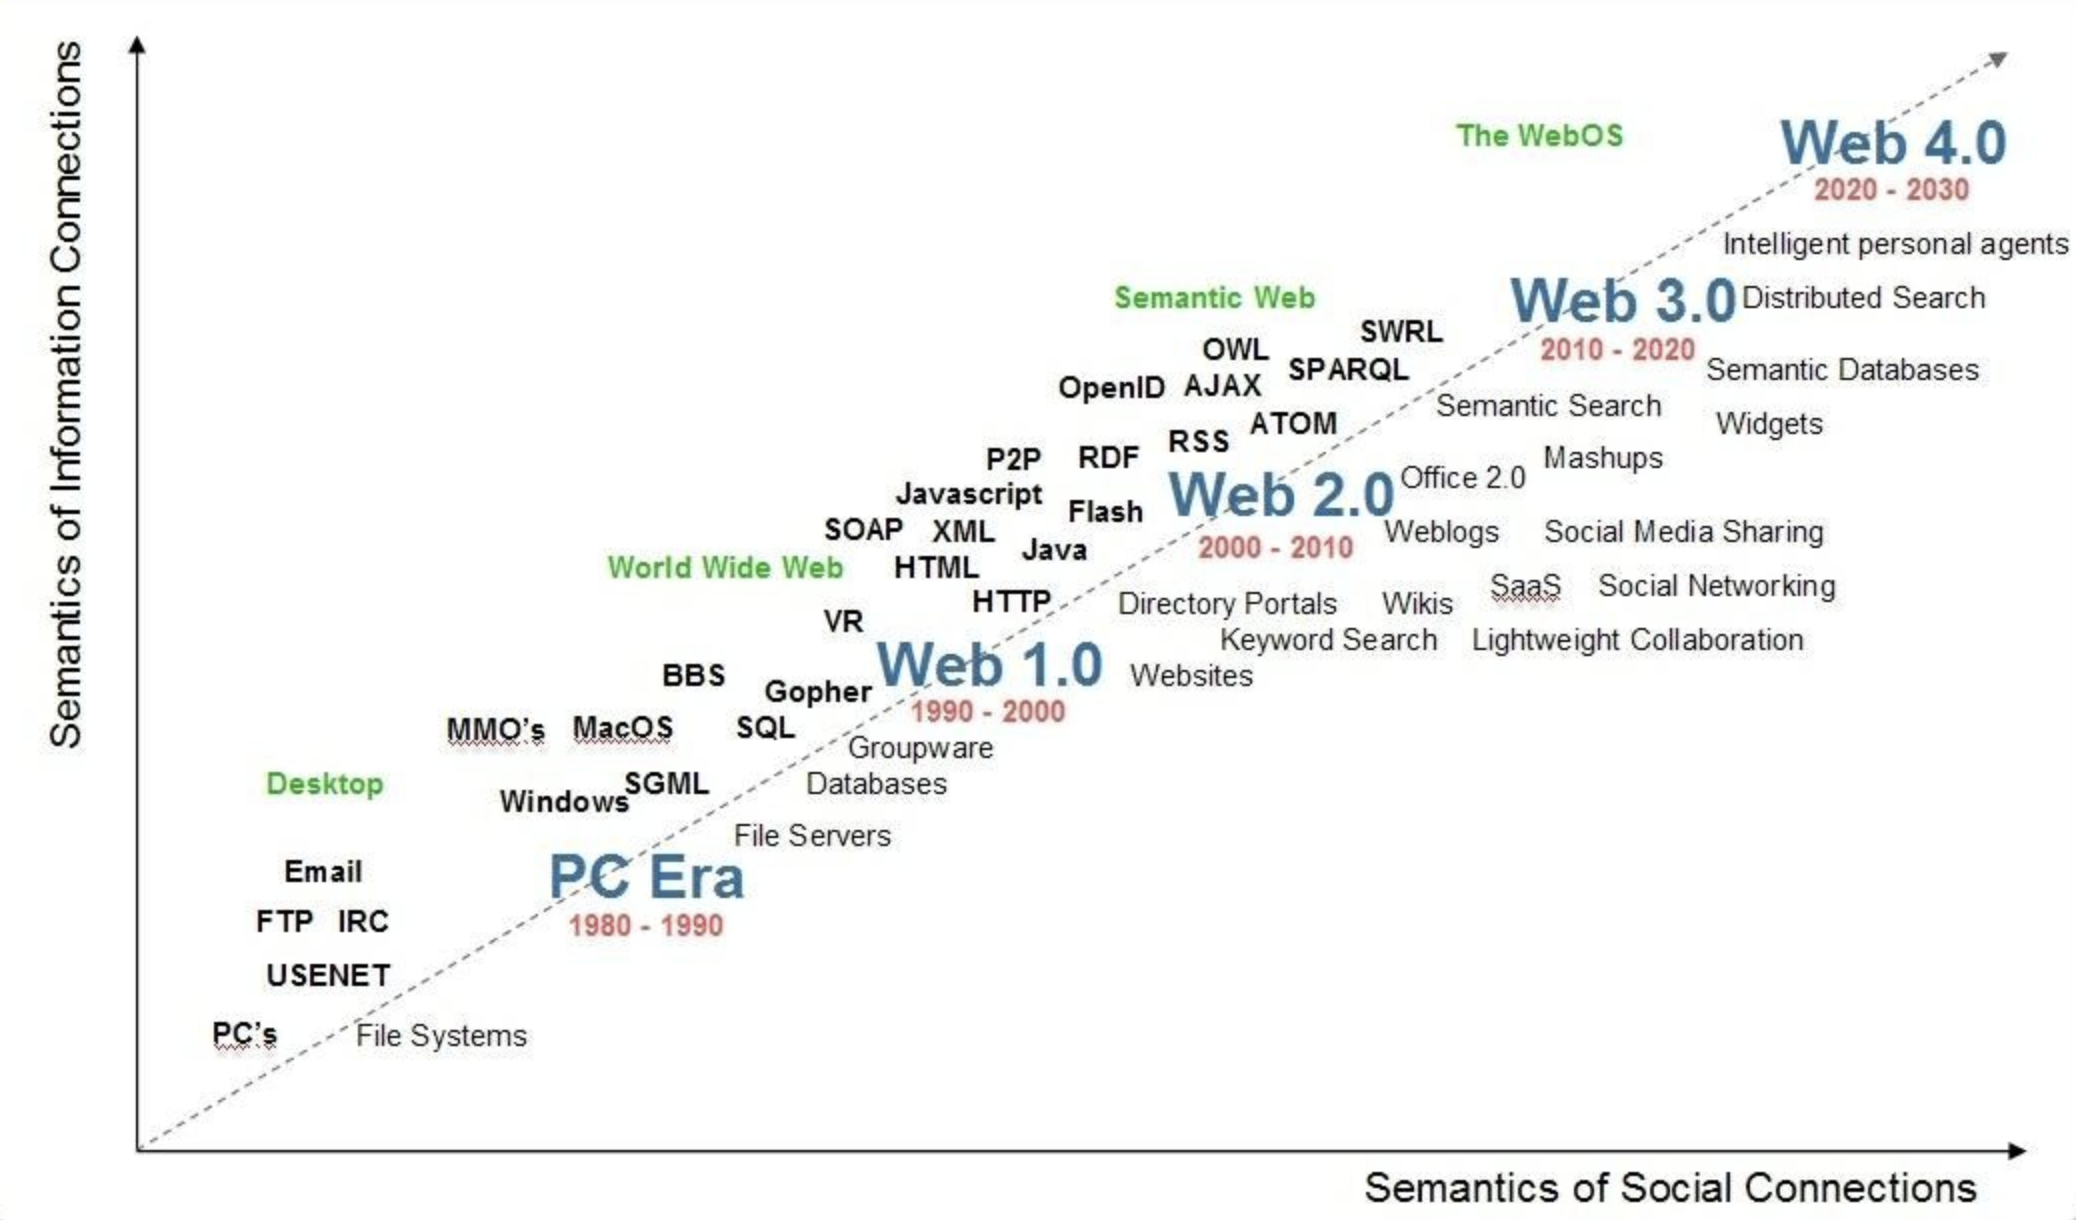
\includegraphics[scale=0.33]{evolucion.png} 
		
		{\scriptsize Tomado de \url{https://www.linkedin.com/pulse/20141119114952-62080297-evolution-of-web-development/}}
		
	\end{frame}
	
	%------------------------------------------------
	% Extra
	\begin{frame}
		
		\frametitle{Extra para ampliar el conocimiento y posibles análisis}
		
		El sitio \url{https://web.archive.org} registra los cambios de ciertos sitios web desde su creación. \\[2mm]
		
		\centering
		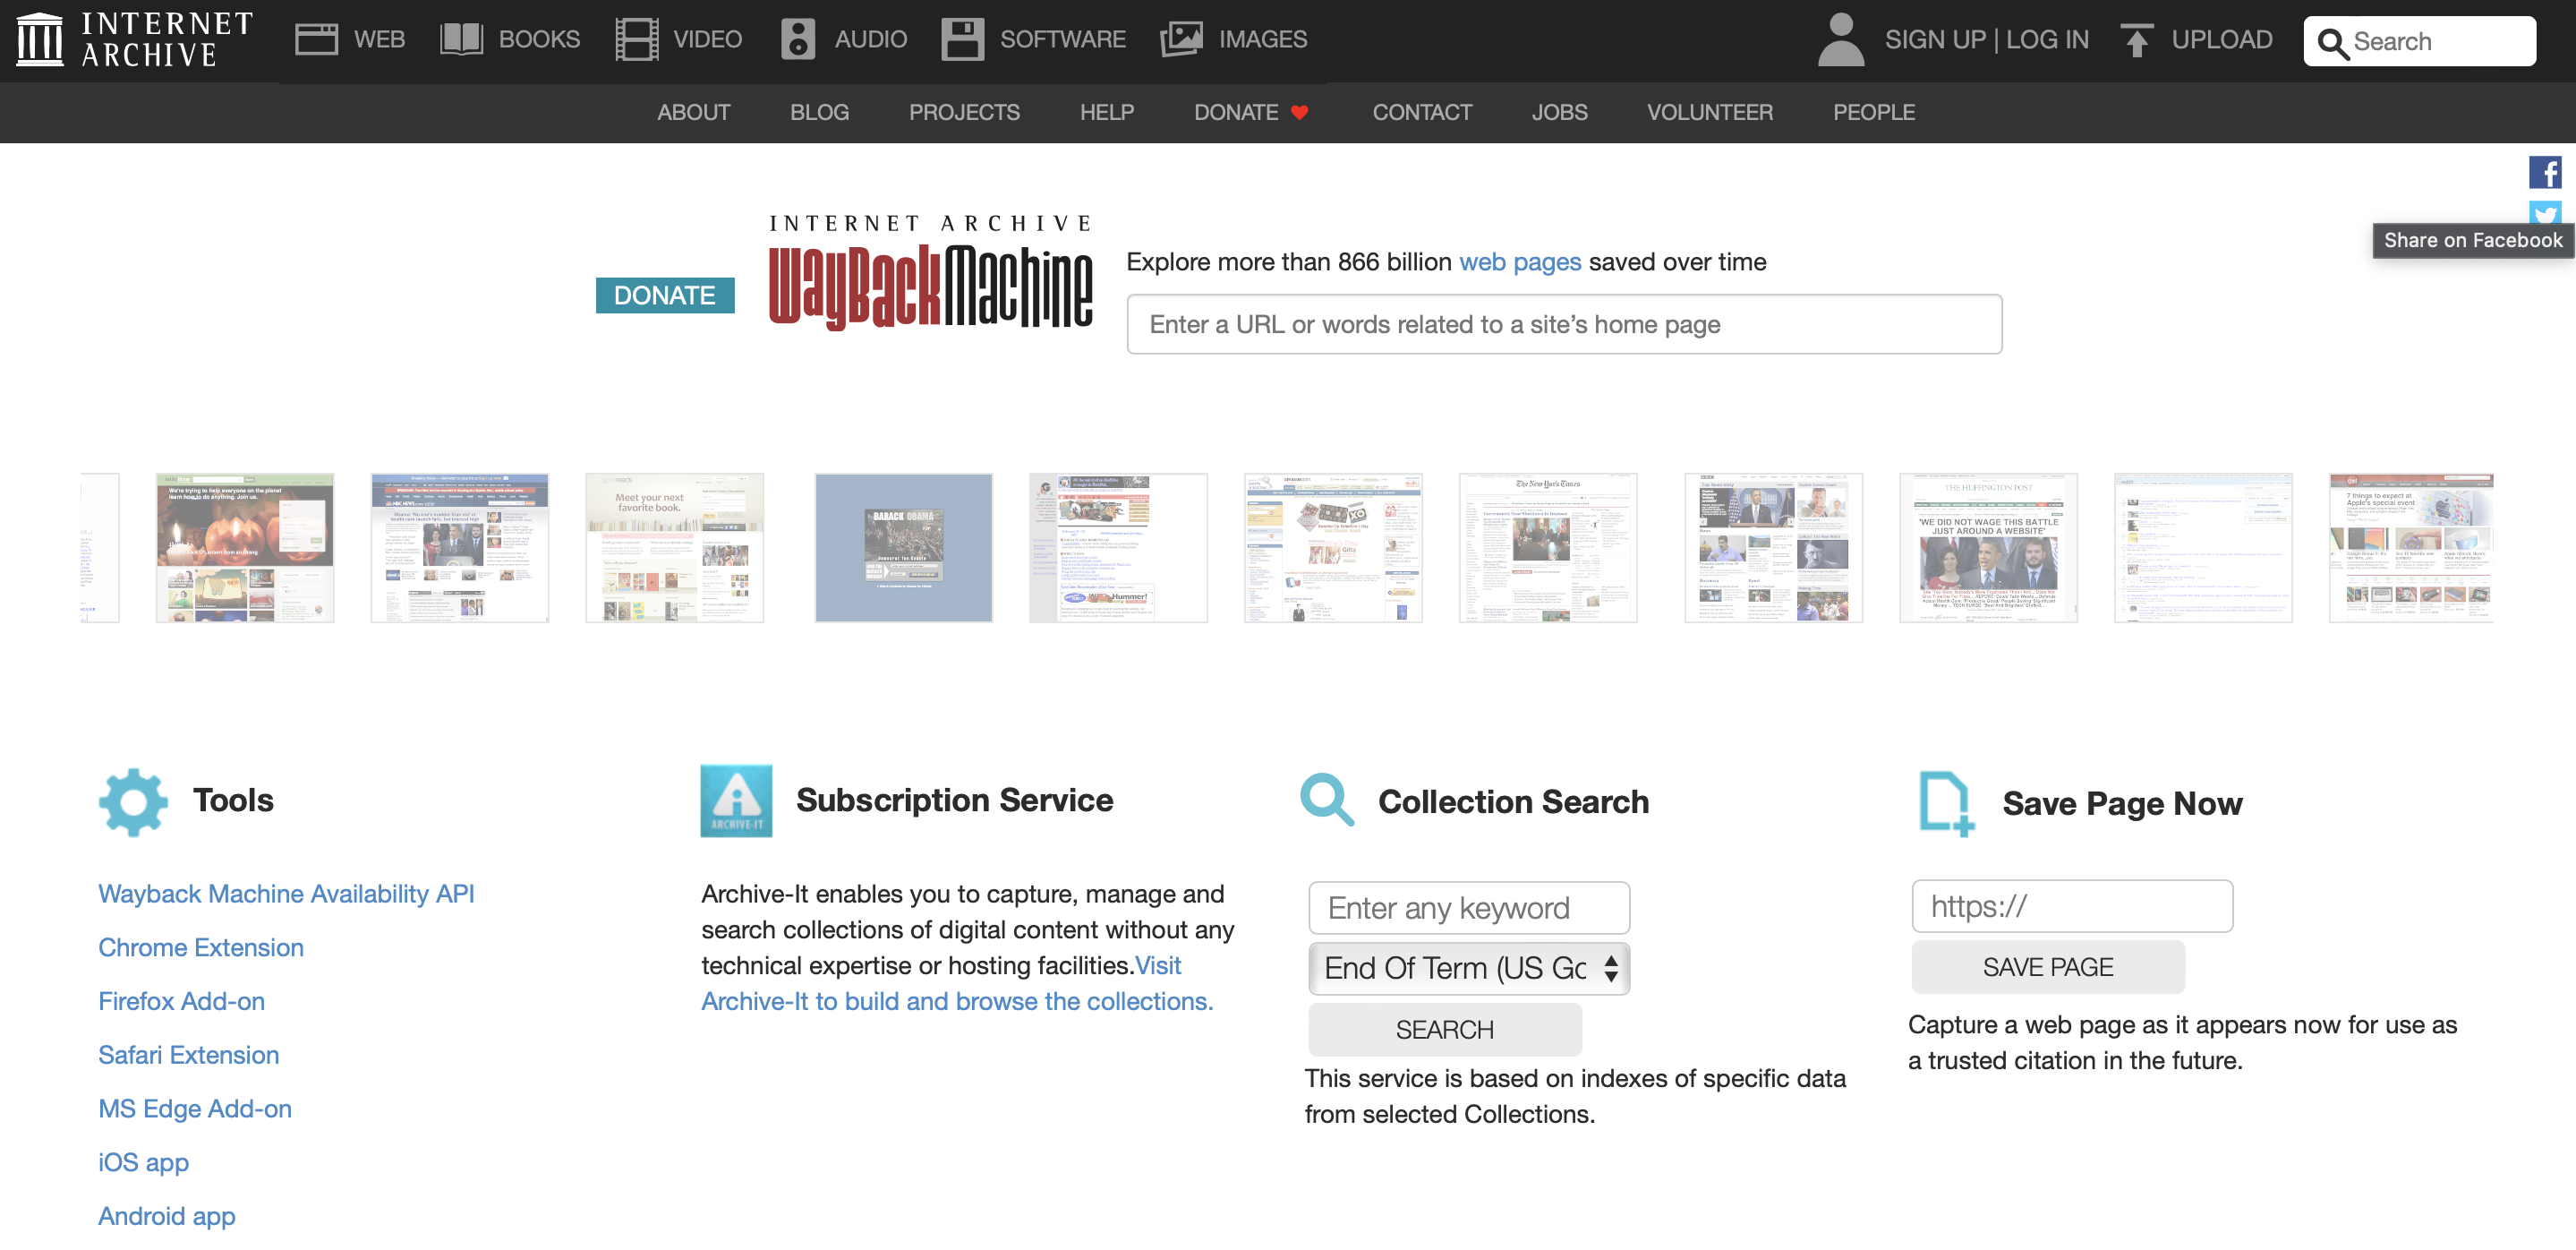
\includegraphics[scale=0.25]{sitio.png} 
		
	\end{frame}
	
	%------------------------------------------------
	% Problemas con los datos en la web actual
	\begin{frame}
		
		\frametitle{Problemas con los datos en la web actual}
		
		\begin{itemize}
			\item Datos distribuidos
			\item Alto porcentaje de datos volátiles
			\item Grandes volúmenes
			\item Datos no estructurados y redundantes
			\item Calidad de los datos
			\item Datos heterogéneos
		\end{itemize}
		
	\end{frame}
	
	%------------------------------------------------
	% Break
	{
		\setbeamertemplate{background canvas}
		{%
			
\includegraphics[width=\paperwidth,height=\paperheight]{meme1.png}
		}
		
		\begin{frame}
		\end{frame}
	}
	
	%------------------------------------------------
	% Problemática
	\begin{frame}
		
		\frametitle{Problema}
		
		Se desea crear un sistema para analizar la opinión con respecto a cierto tema. Las opiniones serán extraídas de varios sitios web y plataformas sociales; algunas se conocen con antelación pero el sistema debe de ser capaz de detectar otros sitios de interés para el análisis y tomar la información que interese procesar. La manera de recopilar la información tiene que ser eficiente. 
		
		\vspace{2\baselineskip}
		
		\textcolor{purple}{
			¿Qué se puede hacer o usar para resolver el problema anterior?
		}
		
		\vspace{3\baselineskip}
		
		\only<2>{
			Se necesita:
			\begin{itemize}
				\item un proceso para rastrear los sitios web de interés y,
				\item un proceso para obtener los datos de los sitios web.
			\end{itemize}
		}
		
	\end{frame}
		
	%------------------------------------------------
	% Web Crawling 
	\begin{frame}
		
		\frametitle{Web Crawling}
		
		\begin{alertblock}{}
			Proceso automatizado de navegar por la web de manera sistemática para indexar y recopilar información de diferentes sitios web.
		\end{alertblock}
		
		\vspace{2\baselineskip}
		
		Tiene como objetivo:
		\begin{itemize}
			\item Recuperar, de manera eficiente y rápida, todos los recursos  ``importantes'' de la web.
		\end{itemize}
		
		\vspace{2\baselineskip}
		
		Los software que realizan la tarea de Web Crawling se les conocen como:
		\begin{itemize}
			\item crawler
			\item spider
			\item walker
		\end{itemize}
		
	\end{frame}
	
	%------------------------------------------------
	% Arquitectura general de un buscador web basado en  crawlers
	\begin{frame}
		
		\frametitle{Arquitectura general de un buscador web basado en  crawlers}
		
	\end{frame}
	
	{
		\setbeamertemplate{background canvas}
		{%
			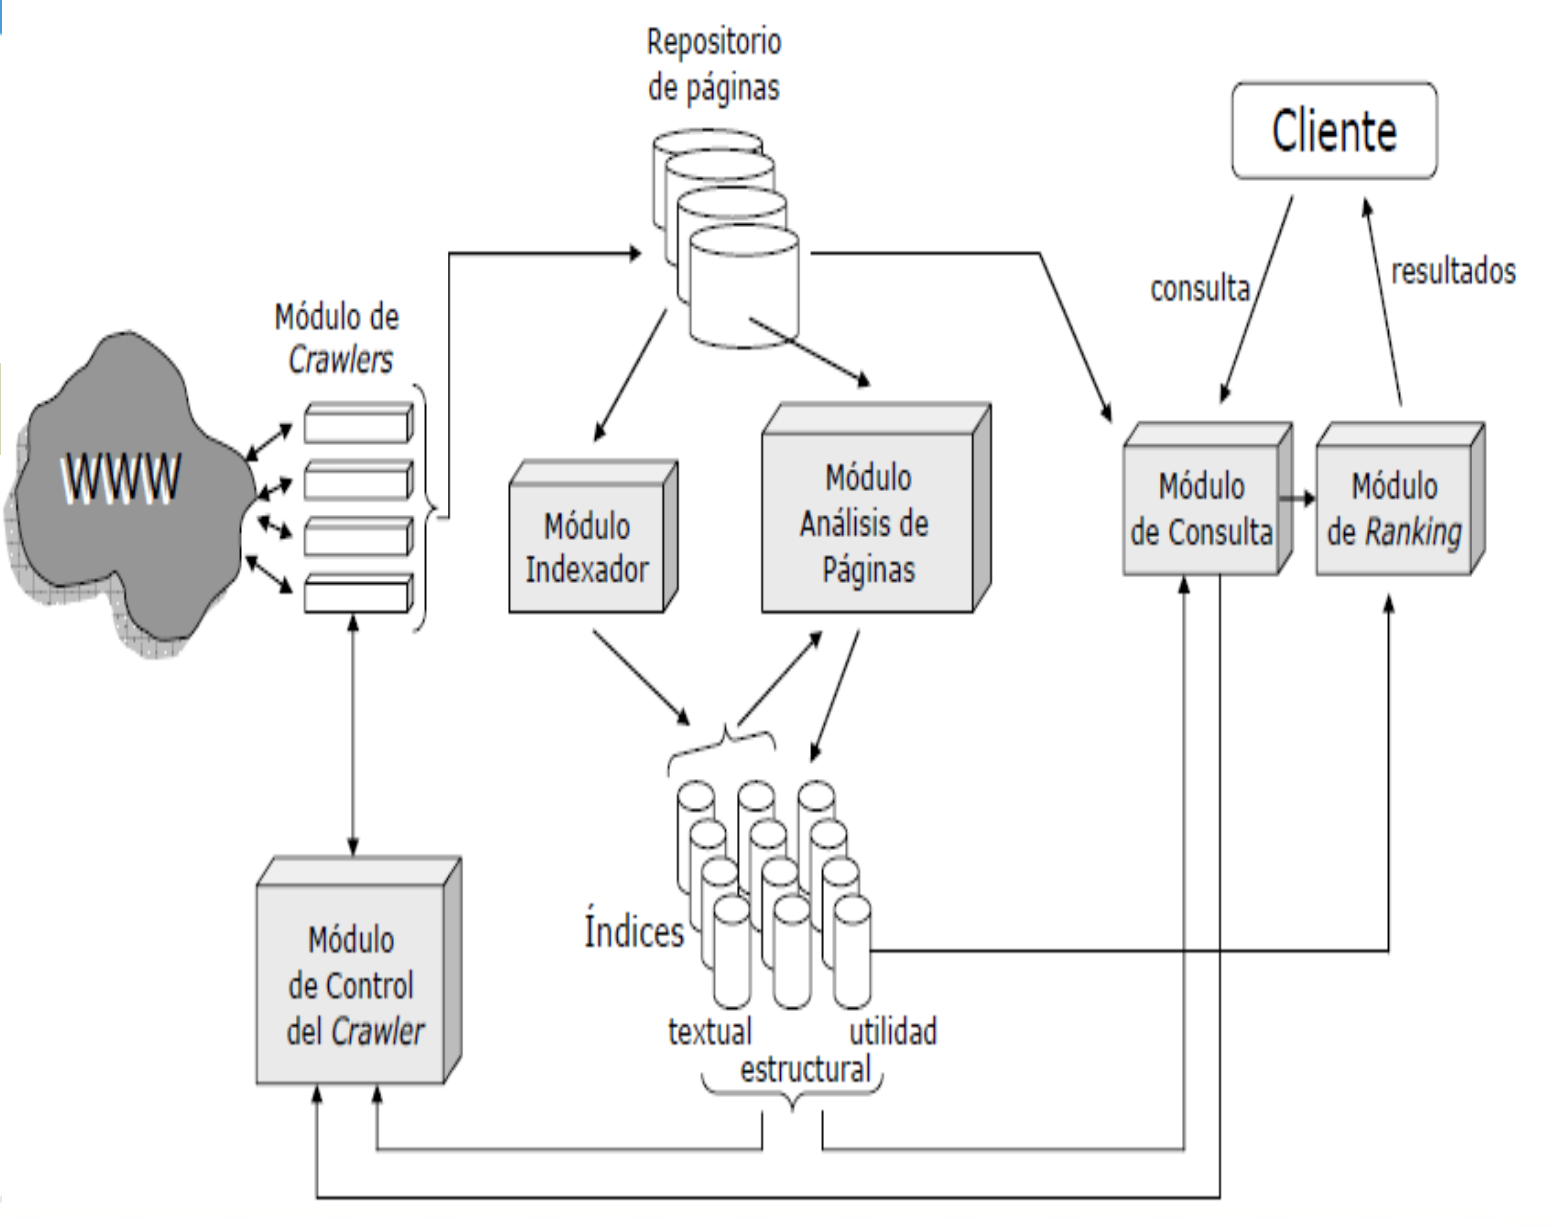
\includegraphics[width=\paperwidth,height=\paperheight]{arquitectura.png}
		}
		
		\begin{frame}
		\end{frame}
	}
	
	%------------------------------------------------
	% Procedimiento del crawler
	\begin{frame}
		
		\frametitle{Procedimiento del crawler}
		
		\centering 
		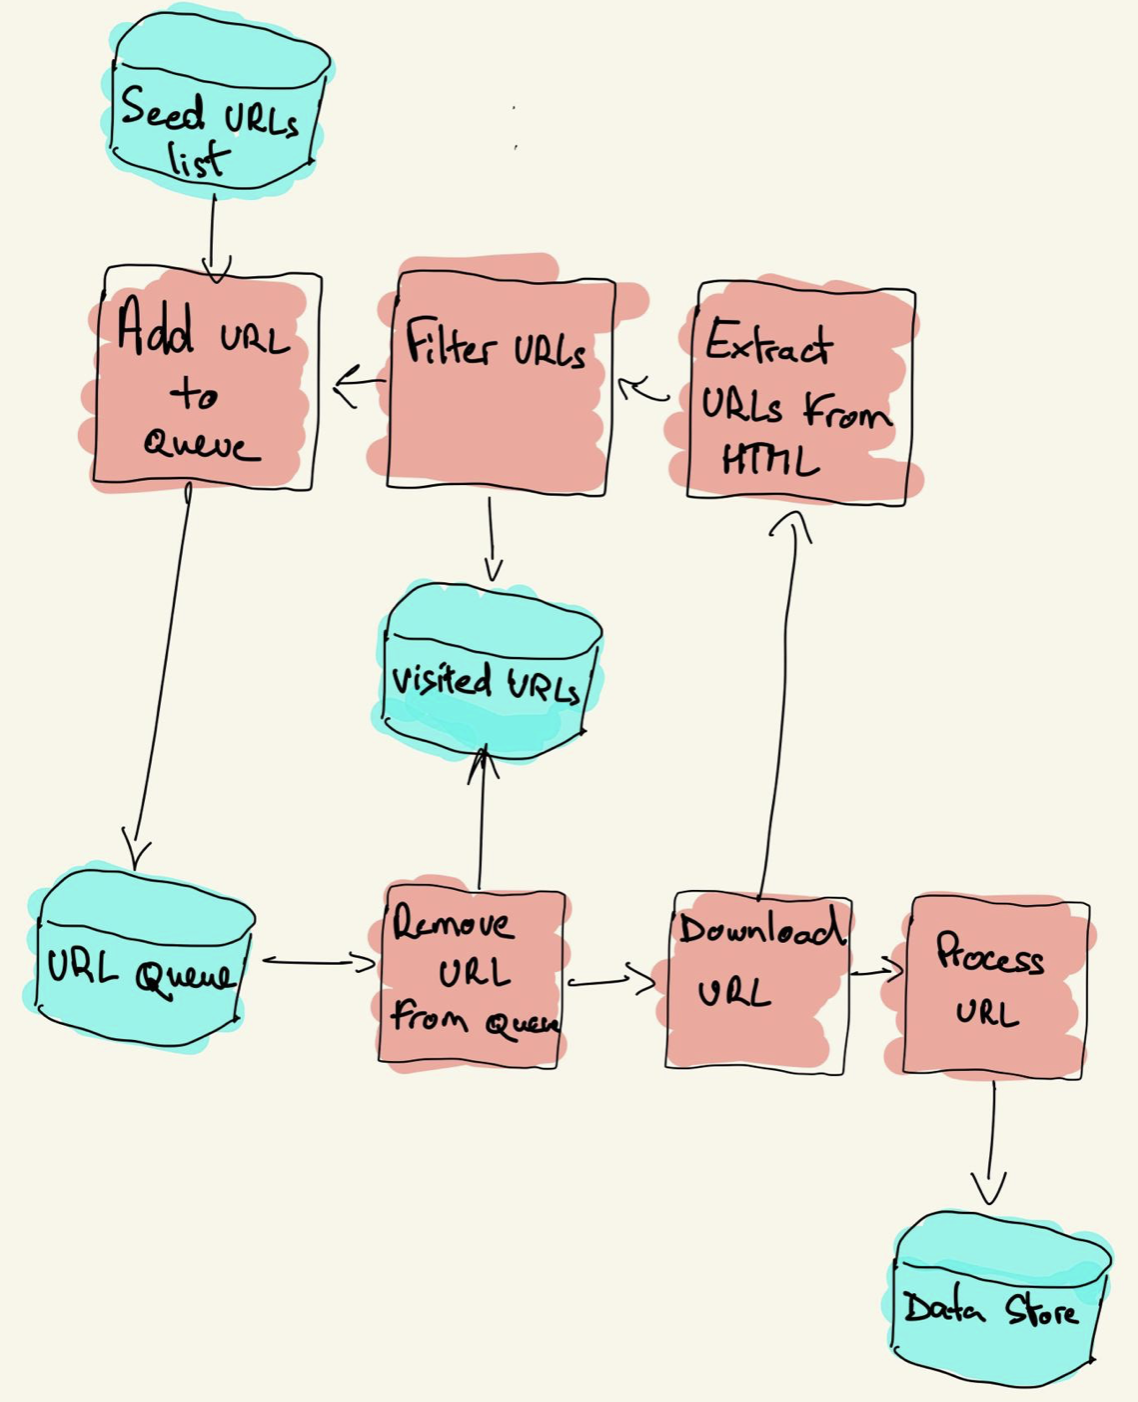
\includegraphics[scale=0.3]{arq-crawler.png}
		
		{\scriptsize Tomado de \url{https://www.scrapingbee.com/blog/crawling-python/}}
		
	\end{frame}
	
	%------------------------------------------------
	% Arquitectura y componentes formales del crawler
	\begin{frame}
		
		\frametitle{Arquitectura y componentes formales del crawler}
		
		\centering 
		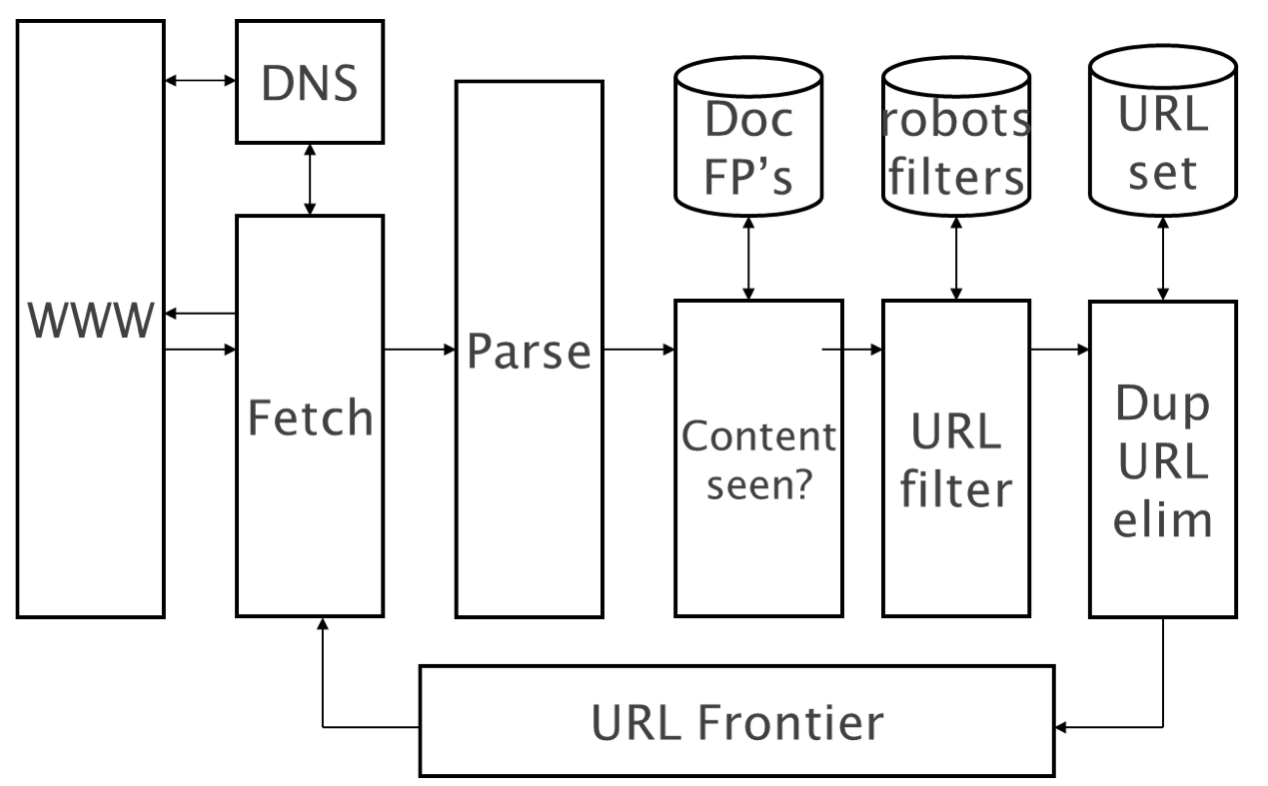
\includegraphics[scale=0.5]{arq-f-crawler.png}
		
		%Componentes
		%	- Url frontera
		%	- DNS
		%	- Módulo de recuperación de páginas 
		%	- Módulo extractor de los datos
		%	- Módulo que determina si una url están en la frontera o fue analizada
		
	\end{frame}
	
	%------------------------------------------------
	% Políticas de los crawlers
	\begin{frame}
		
		\frametitle{Políticas de los crawlers}
		
		Sobre el funcionamiento de los crawlers se definien ciertas reglas o políticas con el objetivo de 
		\begin{itemize}
			\item Optimizar los recursos de red y
			\item Evitar la saturación de los servidores.
		\end{itemize} 
		
		\vspace{2\baselineskip}
		
		Políticas usadas:
		\begin{itemize}
			\item Políticas de amabilidad
			\item Políticas de ordenación de URL
			\item Políticas de revisitado
		\end{itemize}
		
	\end{frame}
	
	%------------------------------------------------
	% Políticas de amabilidad
	\begin{frame}
		
		\frametitle{Políticas de amabilidad}
		
		Las políticas de amabilidad, conocidas también como \textbf{políticas de rastreo}, son reglas establecidas en los sitios web para regular el comportamiento de los web crawlers.
		
		\vspace{2\baselineskip}
		
		Reglas:
		\begin{itemize}
			\item Frecuencia de rastreo 
			%Establecer un límite en la frecuencia con la que un crawler puede acceder a un sitio web dentro de un período de tiempo determinado.
			
			\item Tiempo de espera entre solicitudes
			%Especificar un tiempo mínimo que el crawler debe esperar entre solicitudes consecutivas al servidor. Esto ayuda a reducir la carga en el servidor y permite que otros usuarios accedan al sitio sin demoras excesivas.
			
			\item Exclusión de ciertas áreas del sitio
			%Algunos sitios pueden especificar partes del sitio que no deben ser rastreadas por los crawlers. Esto se logra mediante el archivo robots.txt, que indica a los crawlers qué áreas del sitio pueden o no pueden rastrear.
			
			\item Identificación del crawler
			%Algunos sitios pueden requerir que los crawlers se identifiquen proporcionando un nombre de agente de usuario o un enlace de contacto para el administrador del crawler. Esto permite que los administradores del sitio se pongan en contacto con los propietarios del crawler en caso de problemas o abuso.
			
		\end{itemize}		
		
	\end{frame}
	
	%------------------------------------------------
	% Políticas de ordenación de url
	\begin{frame}
		
		\frametitle{Políticas de ordenación de URL}
		
		Reglas utilizadas para determinar el orden en el que se acceden a las URLs durante el proceso de rastreo y actúa directamente en la eficiencia del rastreo y en garantizar que los recursos del servidor se utilicen de manera efectiva.
		
		\vspace{\baselineskip}
		
		Algunas de las reglas más utilizadas son:
		\begin{itemize}
			
			\begin{minipage}[t]{0.43\textwidth} % Primera columna
				
				\item Aleatoriamente
				
				\item FIFO (First In, First Out)
				
				\item LIFO (Last In, First Out)
				
				\item Backlink Count
				%Recorre primero las páginas de la lista de espera que tienen más referencias de entrada.
	
			\end{minipage}
			\hfill  % Espacio entre las columnas
			\begin{minipage}[t]{0.43\textwidth} % Segunda columna
				
				\item Weighted Backlink Count
				%Es una variante de la política de "Backlink Count" que asigna un peso específico a los backlinks basado en ciertos criterios.
				
				\item Batch PageRank
				%Se basa en el algoritmo PageRank para determinar la prioridad de rastreo de las URL
				
				\item PageRank
				
				\item Focused Crawling
				%Recorre las páginas en función de una búsqueda focalizada a temas predefinidos.
				
			\end{minipage}
			
		\end{itemize}
				
	\end{frame}
		
	%------------------------------------------------
	% Políticas de revisitado
	\begin{frame}
		
		\frametitle{Políticas de revisitado}
		
		Estas reglas definen cuándo y con qué frecuencia de visitan nuevamente las URLs.
		
		\vspace{2\baselineskip}
		
		\begin{itemize}
			\item Uniforme
			% Revisita todas las páginas con la misma periodicidad independientemente de su frecuencia de cambio. 
			
			\item Proporcional (computa previamente métricas)
			% Revisita más las páginas con mayor frecuencia de cambio. Es decir, la frecuencia de visita es proporcional al estimado de actualizaciones de la página.
		\end{itemize}
		
	\end{frame}
	
	%------------------------------------------------
	% Medidas para volver a rastrear
	\begin{frame}
		
		\frametitle{Medidas para volver a rastrear una URL}
		
		\begin{itemize}
			
			\item Edad
			\begin{itemize}
				\item Se refiere al tiempo que ha transcurrido desde que fue descubierta la URL por primera vez por el crawler o desde su última visita.
				\item Se calcula como:
				
				\begin{equation}
					Ep(url) = \left\{
					\begin{aligned}
						0 & \quad \text{si la URL no ha sido modificada} \\
						fecha\_actual - ultima\_visita\_a(url) & \quad \text{e.o.c.}
					\end{aligned} \nonumber
					\right.
				\end{equation}
				
			\end{itemize}
			
			\item Frescura
			\begin{itemize}
				\item Se refiere a la frecuencia con la que se actualiza el contenido de la página y la importancia de las actualizaciones recientes.
				\item Se calcula como:
				
				\begin{equation}
					Fp(url) = \left\{
					\begin{aligned}
						1 & \quad \text{si el continido de la URL es el mismo al almacenado} \\
						0 & \quad \text{e.o.c.}
					\end{aligned} \nonumber
					\right.
				\end{equation}
				
			\end{itemize}
			
		\end{itemize}
		
	\end{frame}
	
	%------------------------------------------------
	% Problemática
	\begin{frame}
		
		\frametitle{Recordando el problema}
		
		Se desea crear un sistema para analizar la opinión con respecto a cierto tema. Las opiniones serán extraídas de varios sitios web y plataformas sociales; algunas se conocen con antelación pero el sistema debe de ser capaz de detectar otros sitios de interés para el análisis y tomar la información que interese procesar. La manera de recopilar la información tiene que ser eficiente. 
		
		\vspace{2\baselineskip}
		
		¿Qué se puede hacer o usar para resolver el problema anterior?
		
		\vspace{3\baselineskip}
		
		Se necesita:
		\begin{itemize}
			\item un proceso para rastrear los sitios web de interés y,
			\item un proceso para obtener los datos de los sitios web.
		\end{itemize}
		
	\end{frame}
	
	%------------------------------------------------
	% Web scraping
	\begin{frame}
		
		\frametitle{Web scraping}
		
		\begin{alertblock}{}
			Proceso de recopilación de datos de páginas web de forma automatizada. 
		\end{alertblock}
		
		\vspace{2\baselineskip}
		
		Utiliza programas de software para analizar y extraer información específica de sitios web, convirtiendo el contenido no estructurado en datos estructurados que pueden ser almacenados y analizados.
		
		\vspace{2\baselineskip}
		
		El web scraping también se conoce como \textbf{extracción de la web}.
		
	\end{frame}
	
	%------------------------------------------------
	% Break 2
	\begin{frame}
		
		\centering
		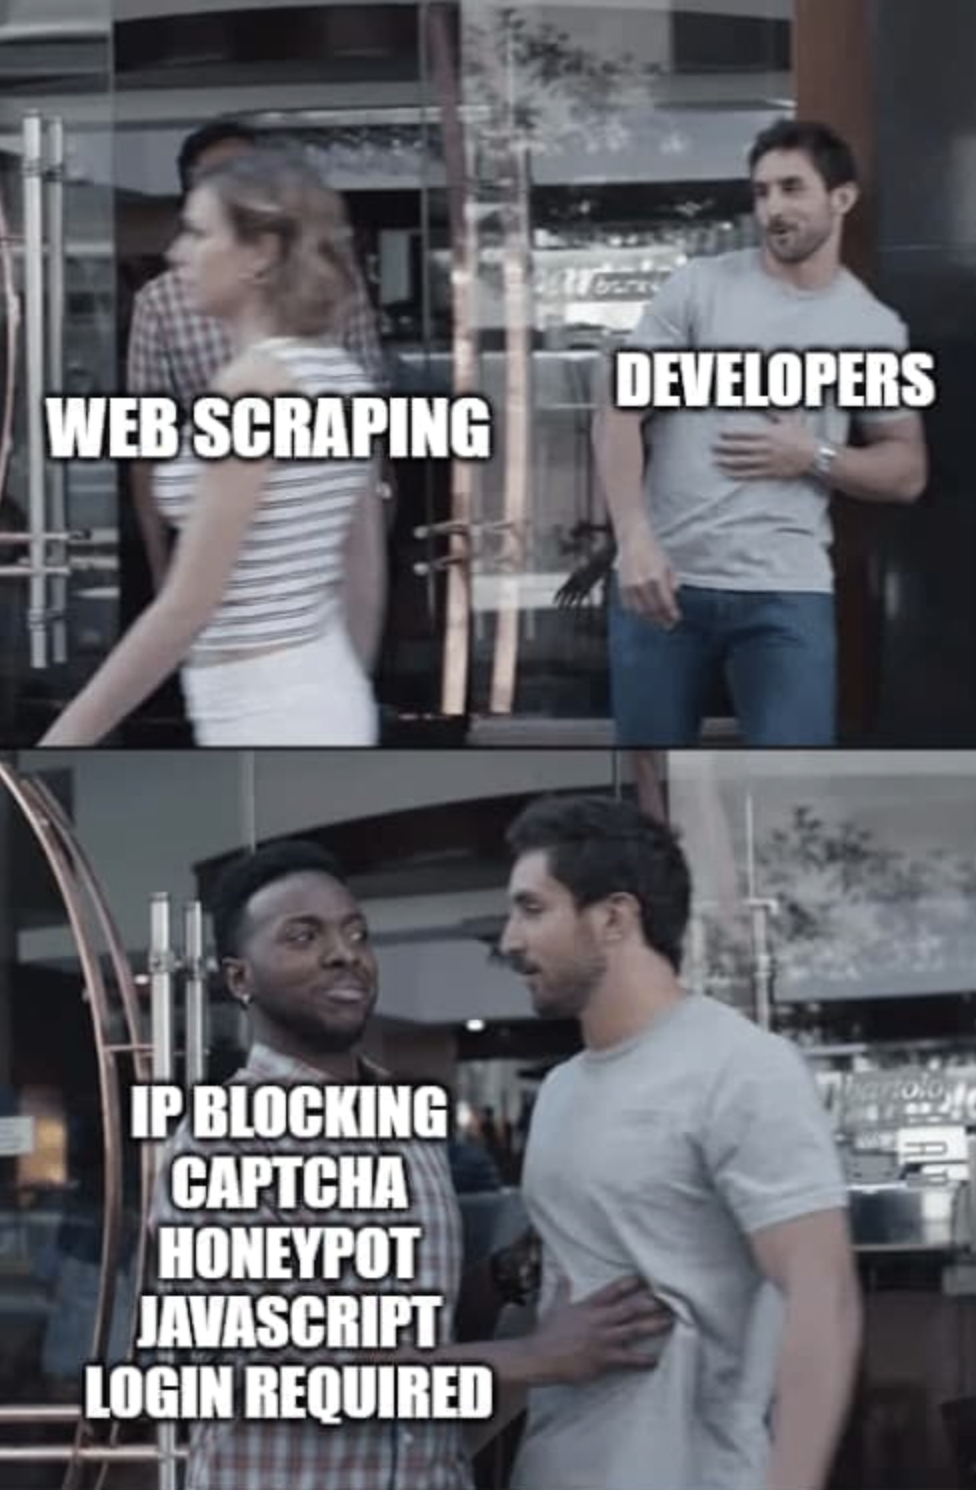
\includegraphics[height=\paperheight]{meme2.png}
		
	\end{frame}
	
	%------------------------------------------------
	% Conclusiones
	\begin{frame}
		
		\frametitle{Conclusiones}
		
		\begin{itemize}
			
			\item La Web está en constante transformación y exige cambios de mentalidad en el diseño e implementación de los recursos que se comparten.
			
			\item La web constituye el mayor repositorio de información por lo que es imprescindible localizar, acceder y recopilar información que satisfaga las necesidades de un usuario. \\[2mm]
			
			\item El crawler y el scraper son herramientas que posibilitan recuperar información en la web. \\[2mm]
			
		\end{itemize}
		
	\end{frame}

	%------------------------------------------------
	% Bibliografía
	\begin{frame}
		
		\frametitle{Bibliografía}
		
		\begin{itemize}
			
			\item Oliva-Santos, R. (2008) Socialización de la información y el conocimiento en la Web. Revista Ciencias Matemáticas. Volumen 24 de 2008. Páginas 93-103.
			
			\item Baeza-Yates, R., Ribeiro-Net, B. (2002)
			Modern Information Retrieval. Páginas 367-395.
			
			\item Manning, Christopher D.;  Raghavan, Prabhakar; Schütze, Hinrich (2007). An Introduction to Information Retrieval. Páginas 399-436.
			
		\end{itemize}
		
	\end{frame}
	
	%------------------------------------------------
	% Fin
	\begin{frame}
		\titlepage
	\end{frame}
	
	
	
\end{document} 